
% --------------------------------------------------------------------
% This is a simple Beamer document that uses beamerthemesigma.sty
% Reading the comments should help you create a presentation even if
% you've never used Beamer before.
% --------------------------------------------------------------------
% Set our document class to Beamer
\documentclass[aspectratio=169]{beamer}

% Some packages for nice font encodings in the final PDF
\usepackage[utf8]{inputenc}
\usepackage[T1]{fontenc}

% From Jeff E
\usepackage{algo}

\usepackage{sigmastyle}

% To insert images
\usepackage{graphicx}

% Useful packages from the AMS
\usepackage{amsmath,amssymb,amsthm}

% Package for code highlighting
\usepackage{minted}
\setminted{linenos=true, breaklines=true, breakanywhere=true, style=default}
\usemintedstyle{monokai}

% Set a title
\title{Grammars Pt. 2}

% The subtitle is generally where I'd expect you to put the week
% number, thus:
\subtitle{Week 4}
% \texorpdfstring to remove compilation warnings if you have math here

% Whoever worked on the presentation:
\author{Anakin}

% A date, if you'd like.
\date{}

% An institute name, if you're so inclined
% \institute{University of Illinois Urbana-Champaign}

% Use the SIGma theme for this Beamer presentation
\usetheme{sigma}
% --------------------------------------------------------------------
% Begin document
\begin{document}

% Beamer calls each slide a "frame", defined within the environment:
% \begin{frame}
%   <frame content here>
% \end{frame}

% This frame is just the title.
\begin{frame}
\titlepage
\end{frame}

% A frame with the table of contents.
% This frame's title is "Outline".
\begin{frame}{Outline}
  \tableofcontents
\end{frame}

% % The frame title is a flag.
% \begin{frame}{Updates!}
%   % Let's put some real content in this frame:
%   Weekly updates:
%   \begin{itemize}
%     \item I have none
%   \end{itemize}
% \end{frame}

% Start a section: *sections* (subsections, etc.) are what show up in the TOC.
\section{Context Free Grammars}
% Section pages can be printed thus:
\frame{\sectionpage}
% There's a way to automate this, see:
% https://tex.stackexchange.com/questions/178800/creating-sections-each-with-title-pages-in-beamers-slides/178803

\begin{frame}{Quick Review}
    $$
        {\LARGE \Set{\texttt{0}^n \texttt{1}^n | n \geq 0}} \text{ is generated by }\pause
    $$
    {
    \LARGE
    \vspace{10pt}
    \begin{align*}
        A ~&\to~ \texttt{0}A\texttt{1} \\
        A ~&\to~ B                     \\
        B ~&\to~ \varepsilon           \\
    \end{align*}
    }
\end{frame}

\begin{frame}{Quick Review}
    $$
        {\LARGE \Set{\texttt{0}^n \texttt{1}^n | n \geq 0}} \text{ is generated by }
    $$
    {
    \LARGE
    \vspace{10pt}
    \begin{align*}
        A ~&\to~ \texttt{0}A\texttt{1} ~|~ \varepsilon \\
    \end{align*}
    }
\end{frame}

\begin{frame}{Determining If Strings Are In A CFL}
    \begin{center}
        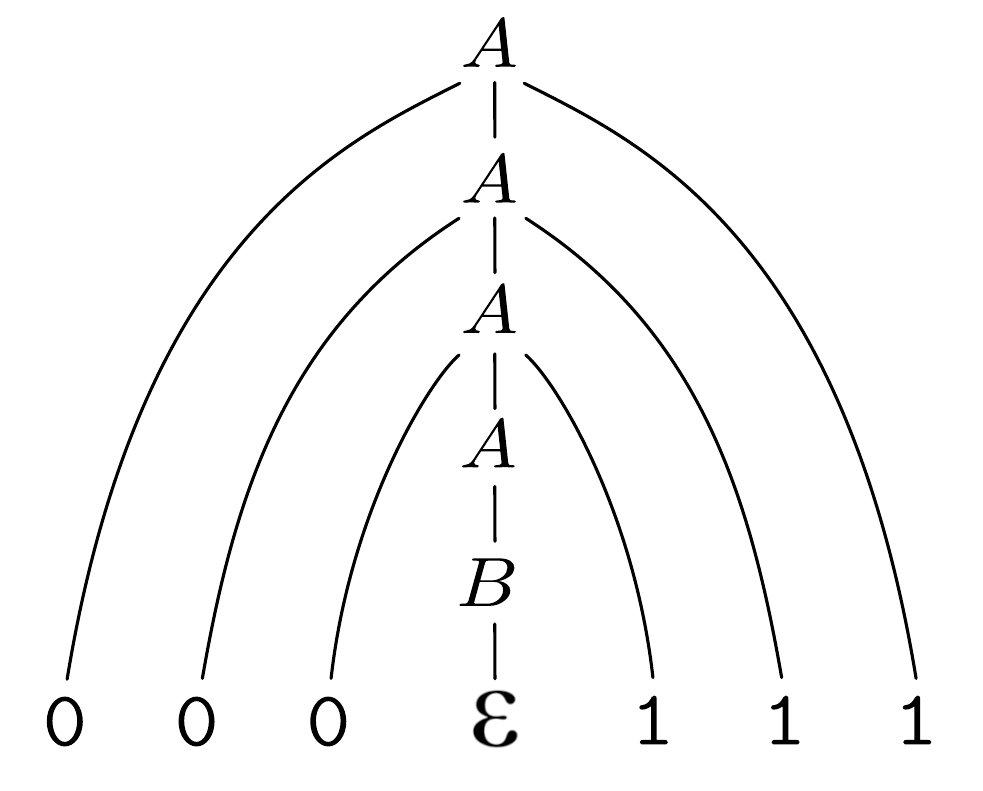
\includegraphics[scale=0.33]{images/CFG_tree.png}
    \end{center}
\end{frame}

\begin{frame}{Determining If Strings Are In A CFL}
    $$
        A \Rightarrow \texttt{0}A\texttt{1} \Rightarrow \texttt{00}A\texttt{11} \Rightarrow \texttt{000}A\texttt{111} \Rightarrow \texttt{000}B\texttt{111} \Rightarrow \texttt{000}\varepsilon\texttt{111} \Rightarrow \texttt{000}\texttt{111}
    $$
\end{frame}

\begin{frame}{Comparison with Regular Languages}
    \begin{itemize}
        \item CFGs define a language much like Regex/DFAs/NFAs \pause
        \item Regex / DFAs / NFAs $\leftrightarrow$ Regular Languages 
        \item Context Free Grammars $\leftrightarrow$ Context Free Languages 
    \end{itemize}
\end{frame}

\begin{frame}{Questions!}
    This is going to be a review of a ton of things we've talked about since automata are coming back \pause
    \begin{itemize}
        \item Create a CFG and NFA / DFA to recognize $\set{w | \text{the length of } w \text{ is odd}}$
        \item Create a CFG to recognize $\set{w | \text{the length of } w \text{ is odd and the middle character is } \texttt{0}}$
    \end{itemize}
\end{frame}

\begin{frame}{Answers}
    Create a CFG and NFA / DFA to recognize $\set{w | \text{the length of } w \text{ is odd}}$
    \begin{center}
        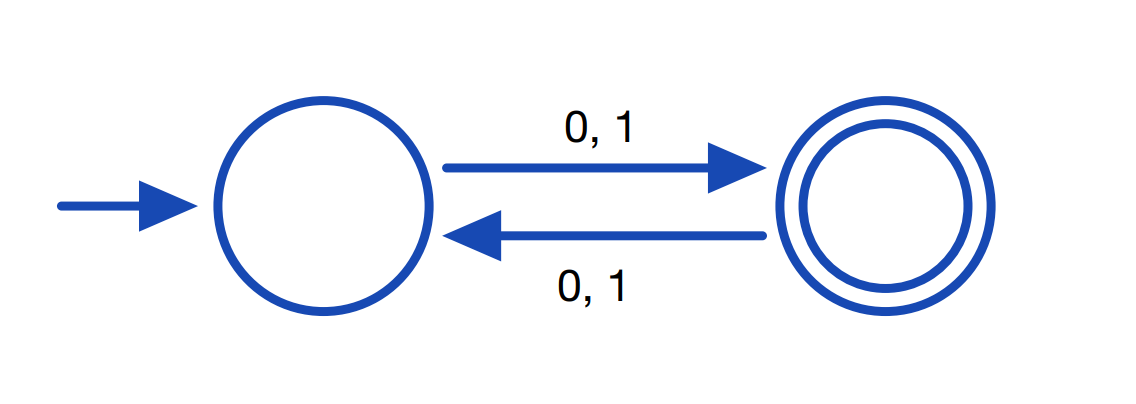
\includegraphics[scale=0.30]{images/odd.png}
    \end{center}
    {
    \Large
    \begin{align*}
        S ~&\to~ \texttt{1}E ~|~ \texttt{0}E \\
        E ~&\to~ \varepsilon ~|~ \texttt{0}S ~|~ \texttt{1}S  \\
    \end{align*}
    }
\end{frame}

\begin{frame}{Answers}
    Create a CFG to recognize $\set{w | \text{the length of } w \text{ is odd and the middle character is } \texttt{0}}$
    {
    \Large
    \begin{align*}
        S ~&\to~ \texttt{0} ~|~ TST \\
        T ~&\to~  \texttt{0} ~|~ \texttt{1} \\
    \end{align*}
    }
\end{frame}

\section{Pushdown Automata}
\frame{\sectionpage}

\begin{frame}{Automata for CFLs}
    \begin{itemize}
        \item {\large Regex $\leftrightarrow$ DFAs / NFAs} \pause
        \item {\large Context Free Grammars $\leftrightarrow$ \textbf{???} }
    \end{itemize}
\end{frame}

\begin{frame}{Automata for CFLs}
    \begin{itemize}
        \item {\large Regex $\leftrightarrow$ DFAs / NFAs}
        \item {\large Context Free Grammars $\leftrightarrow$ \textbf{Pushdown Automata}}
    \end{itemize}
\end{frame}

\begin{frame}{State Machines With an Upgrade}
    \begin{center}
        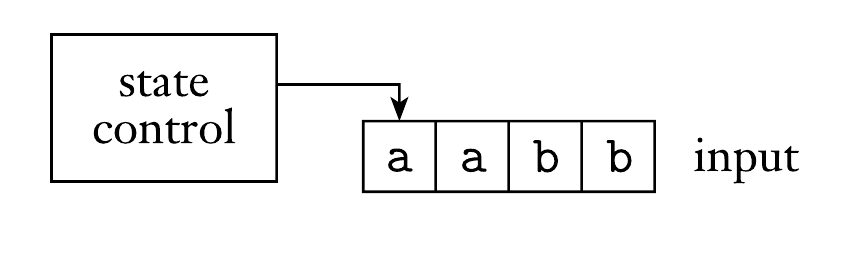
\includegraphics[scale=0.33]{images/finite_automata.png}
    \end{center}
\end{frame}

\begin{frame}{State Machines With an Upgrade}
    \begin{center}
        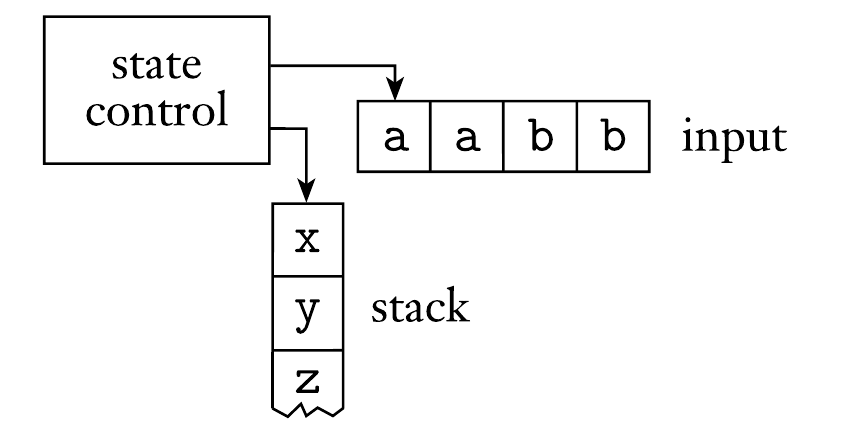
\includegraphics[scale=0.33]{images/pushdown_automata.png}
    \end{center}
\end{frame}

\begin{frame}{What is a Stack??}
    \begin{itemize}
        \item Think about stacking objects (books, plates, whatever) \pause
        \item You can add items to the \textbf{top only} and lose immediate access to anything below it \pause
        \item If you want to get an item from your stack, you have to pick up the \textbf{top item first} and then discard it
    \end{itemize}
\end{frame}

\begin{frame}{Stack}
    \begin{center}
        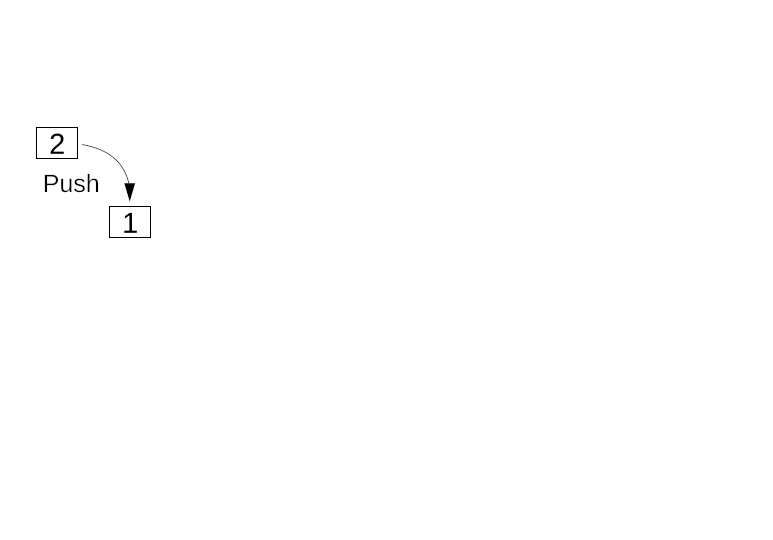
\includegraphics[scale=0.4625]{images/stack/Stack_1.png}
    \end{center}
\end{frame}

\begin{frame}{Stack}
    \begin{center}
        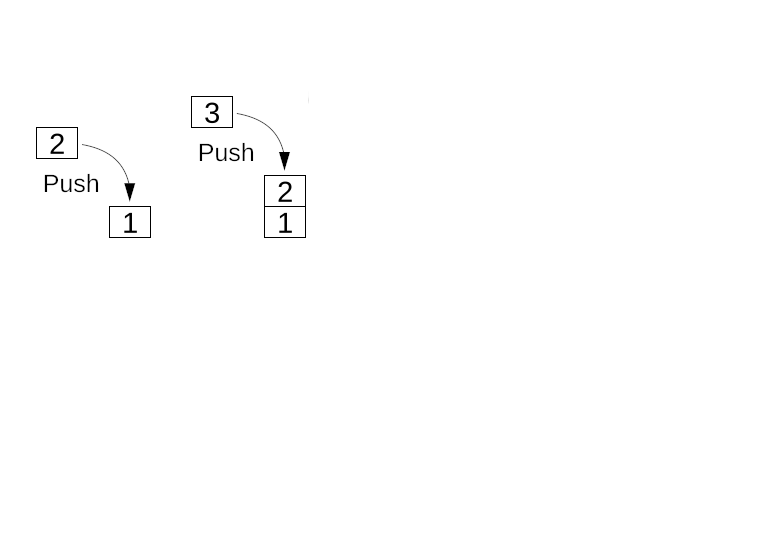
\includegraphics[scale=0.4625]{images/stack/Stack_2.png}
    \end{center}
\end{frame}

\begin{frame}{Stack}
    \begin{center}
        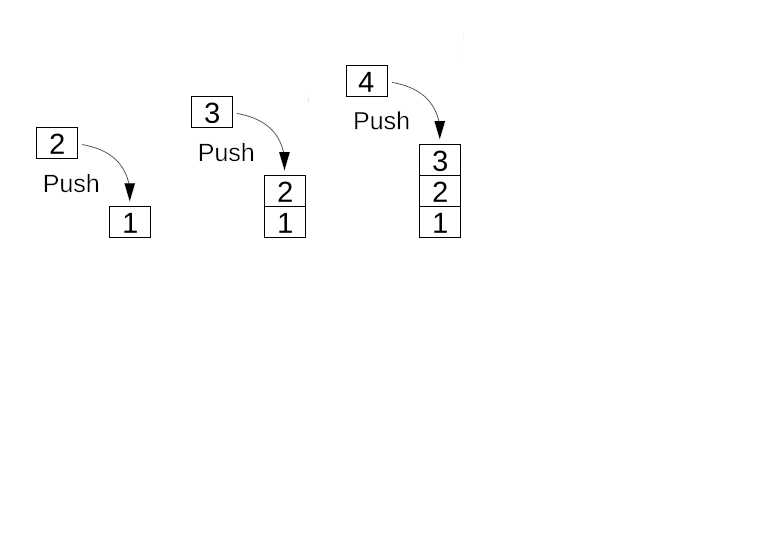
\includegraphics[scale=0.4625]{images/stack/Stack_3.png}
    \end{center}
\end{frame}

\begin{frame}{Stack}
    \begin{center}
        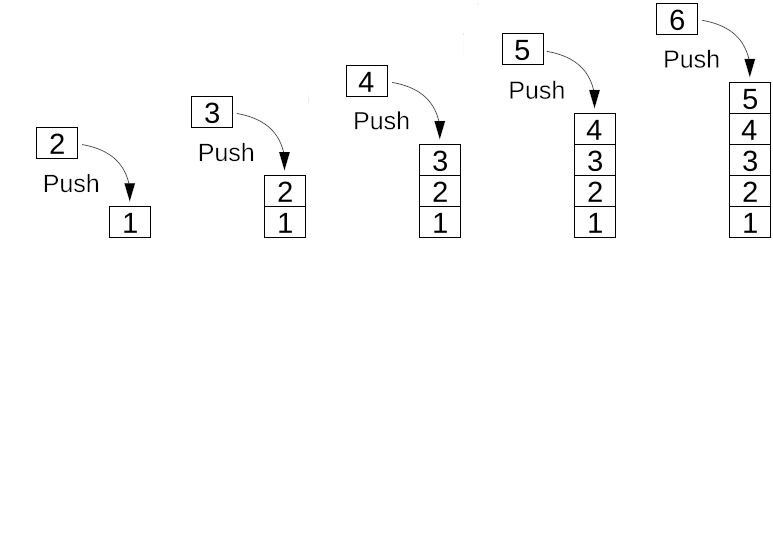
\includegraphics[scale=0.4625]{images/stack/Stack_4.png}
    \end{center}
\end{frame}

\begin{frame}{Stack}
    \begin{center}
        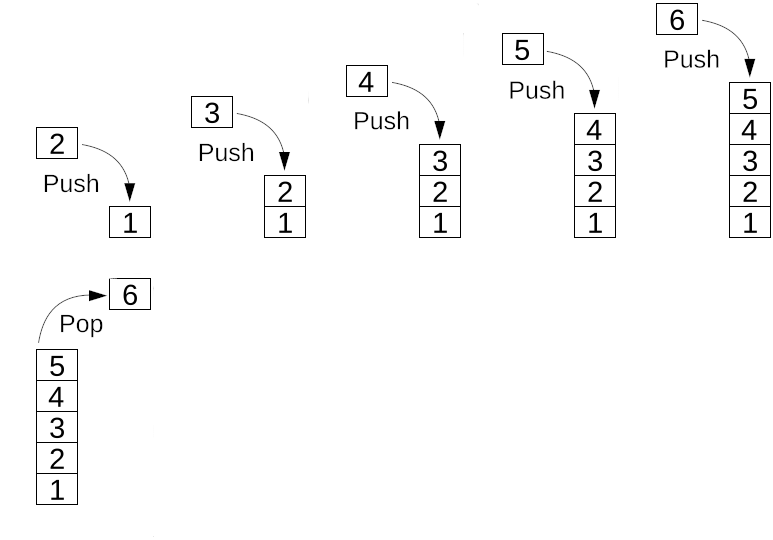
\includegraphics[scale=0.4625]{images/stack/Stack_5.png}
    \end{center}
\end{frame}

\begin{frame}{Stack}
    \begin{center}
        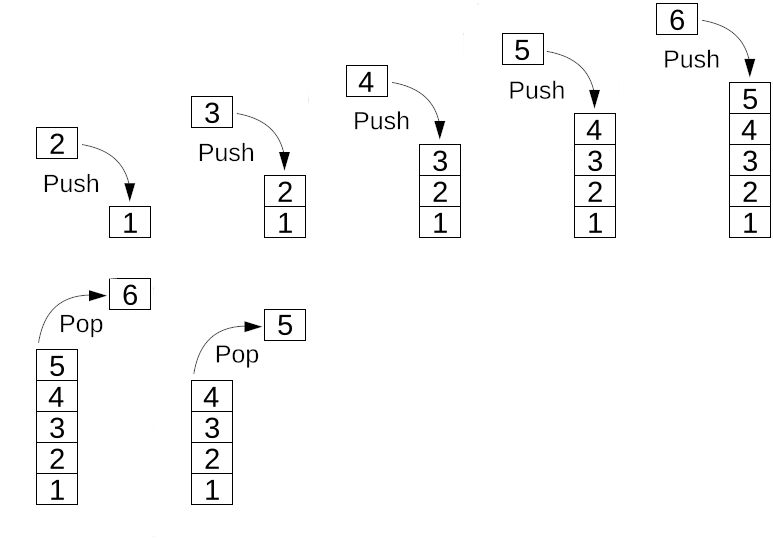
\includegraphics[scale=0.4625]{images/stack/Stack_6.png}
    \end{center}
\end{frame}

\begin{frame}{Stack}
    \begin{center}
        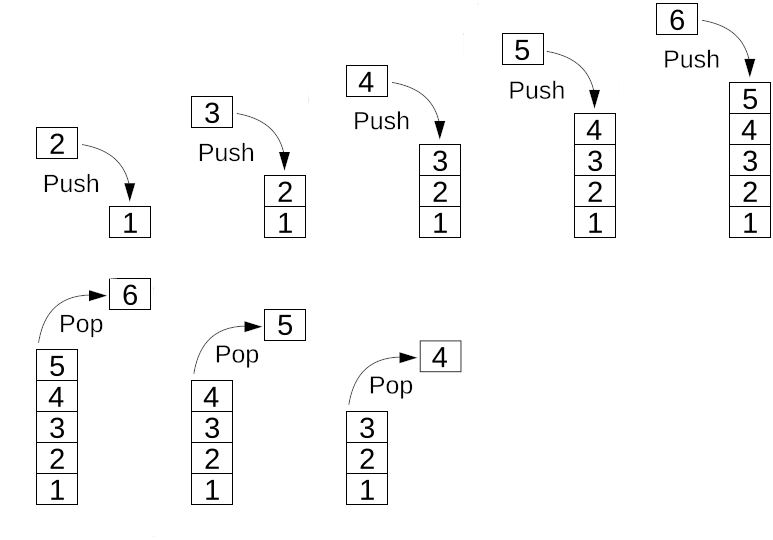
\includegraphics[scale=0.4625]{images/stack/Stack_7.png}
    \end{center}
\end{frame}

\begin{frame}{Stack}
    \begin{center}
        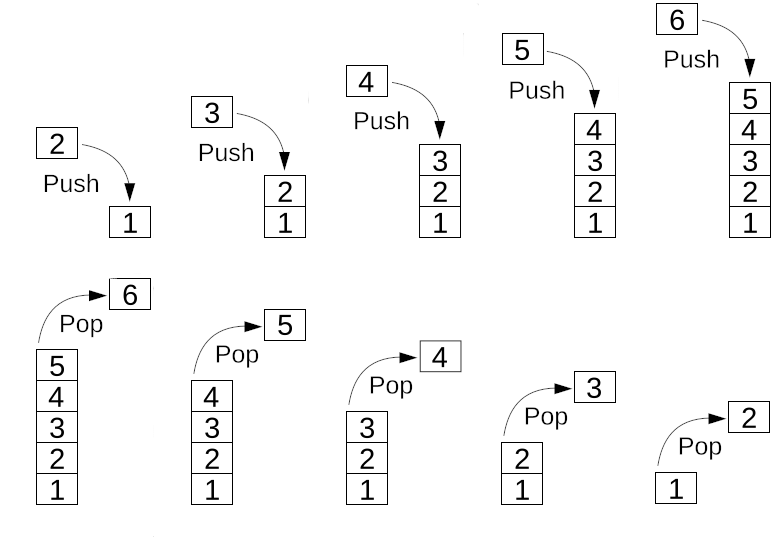
\includegraphics[scale=0.4625]{images/stack/Stack_8.png}
    \end{center}
\end{frame}

\begin{frame}{What does this get you?}
    \begin{itemize}
        \item You remember DFAs and NFAs??? \pause
        \item We could remember only the \textbf{current state} \pause
        \item The stack gives us a sort of \textbf{memory} \pause
        \item NFA + Stack $\leftrightarrow$ Context Free Grammar
    \end{itemize}
\end{frame}

\begin{frame}{DFA}
    \begin{center}
        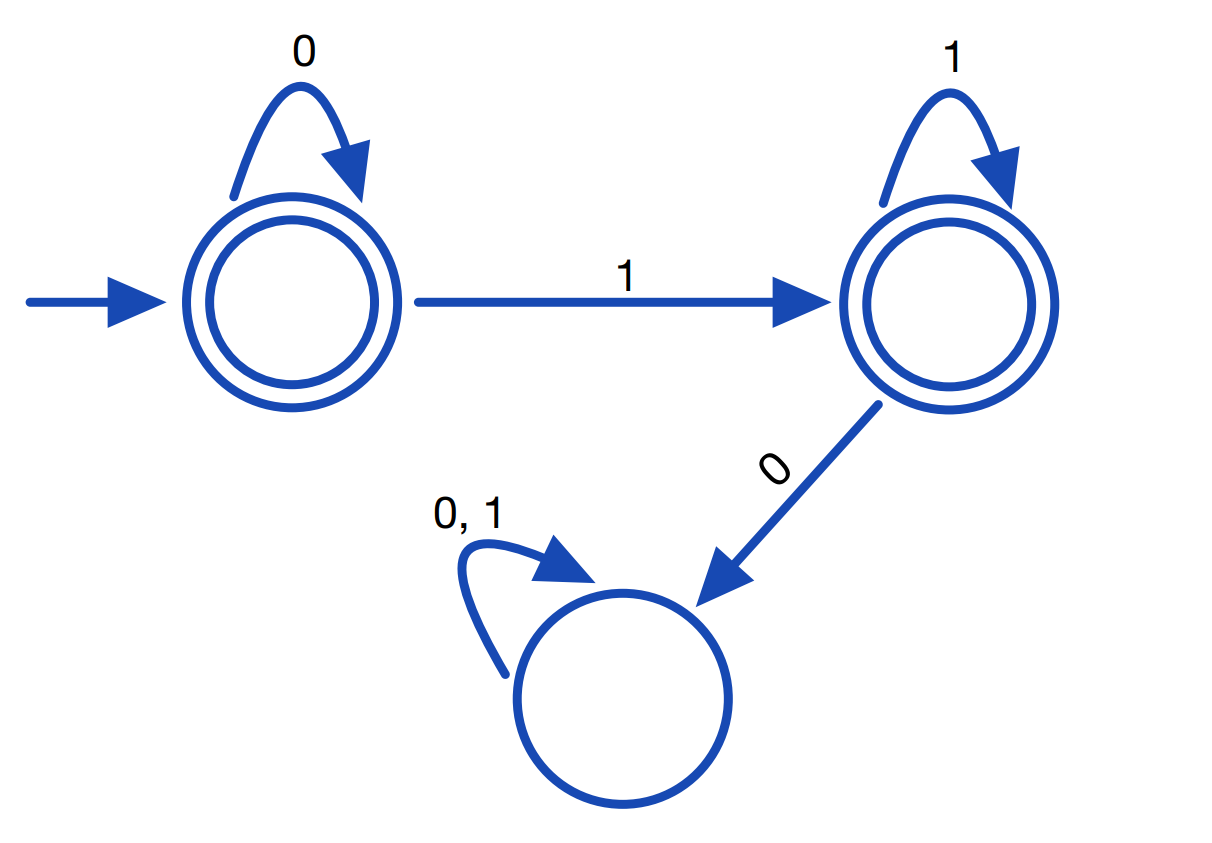
\includegraphics[scale=0.30]{images/01.png}
    \end{center}
\end{frame}

\begin{frame}{PDA for $\Set{0^n 1^n,\ n \geq 0}$}
    \begin{center}
        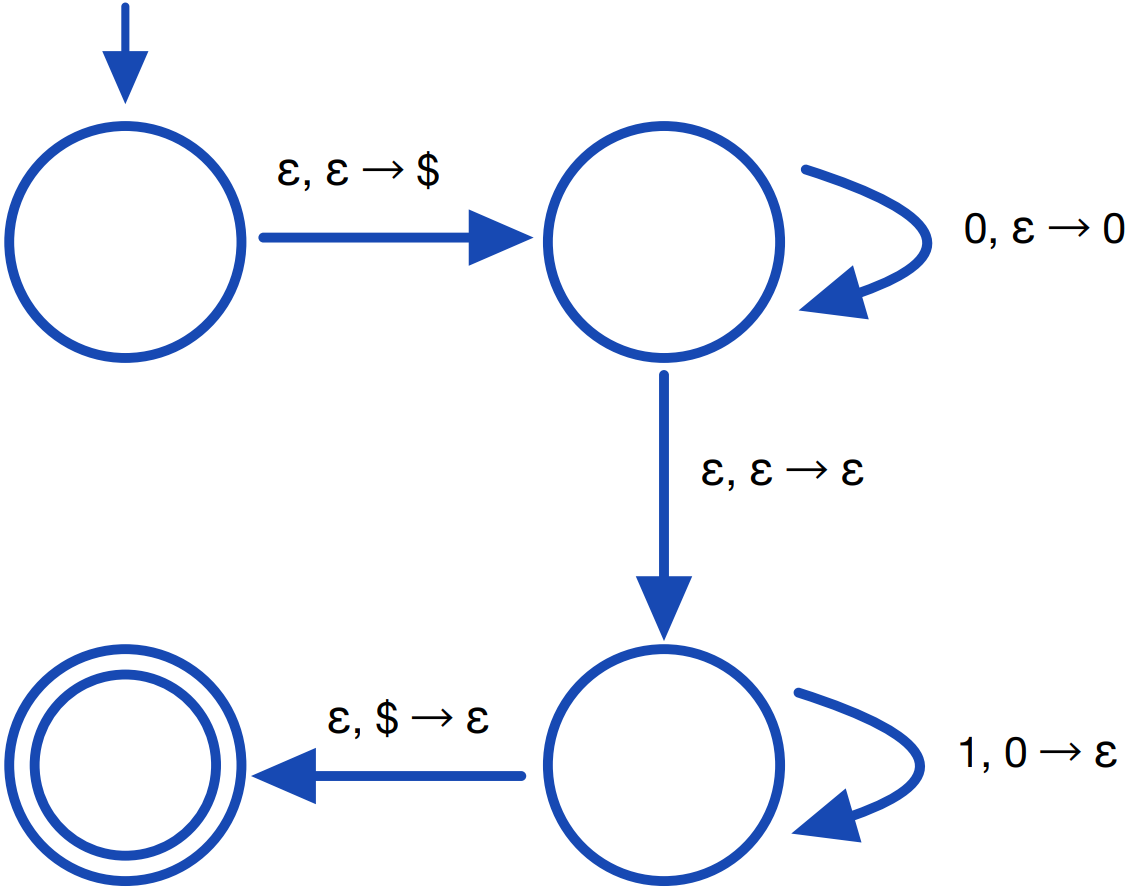
\includegraphics[scale=0.30]{images/PDA_1.png}
    \end{center}
\end{frame}

\begin{frame}{PDA for $\Set{0^n 1^n,\ n \geq 0}$}
    \begin{center}
        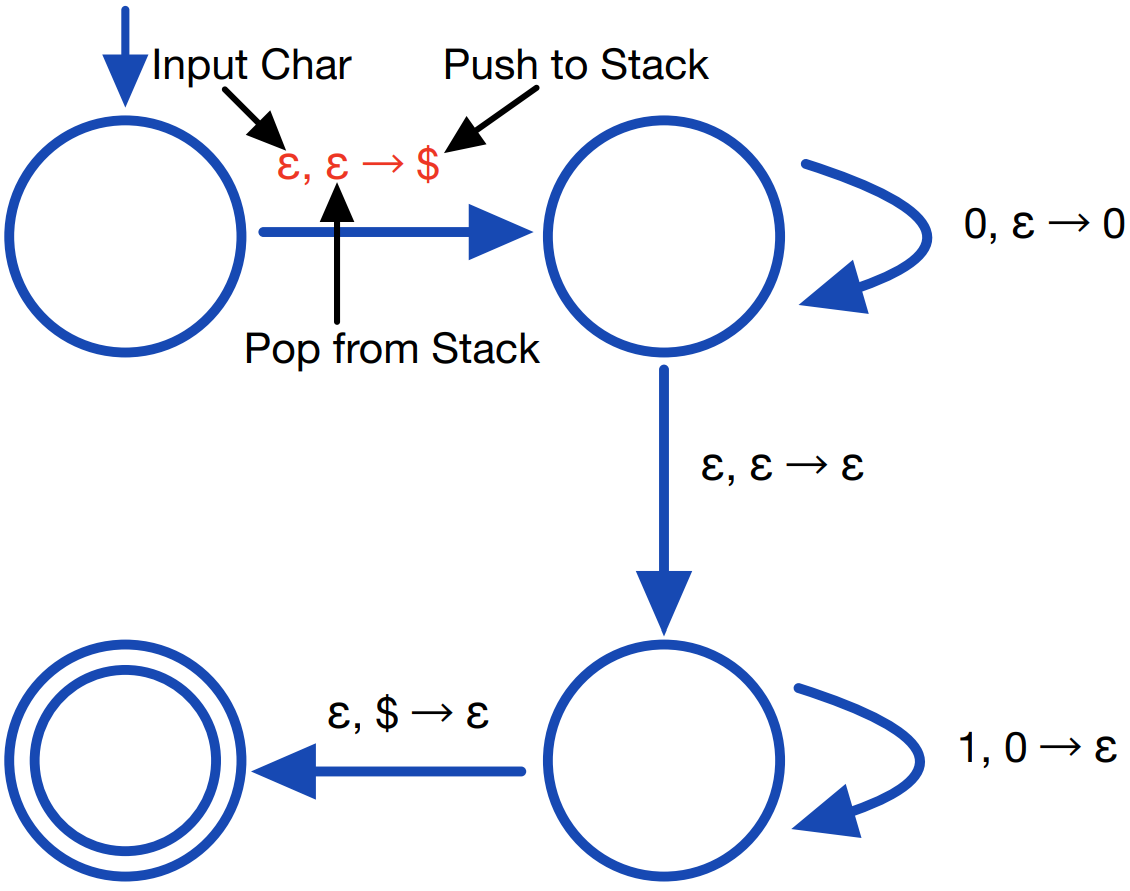
\includegraphics[scale=0.30]{images/PDA_2.png}
    \end{center}
\end{frame}

\begin{frame}{$\texttt{0011} \stackrel{?}{\in} \Set{0^n 1^n,\ n \geq 0}$}
    \begin{center}
        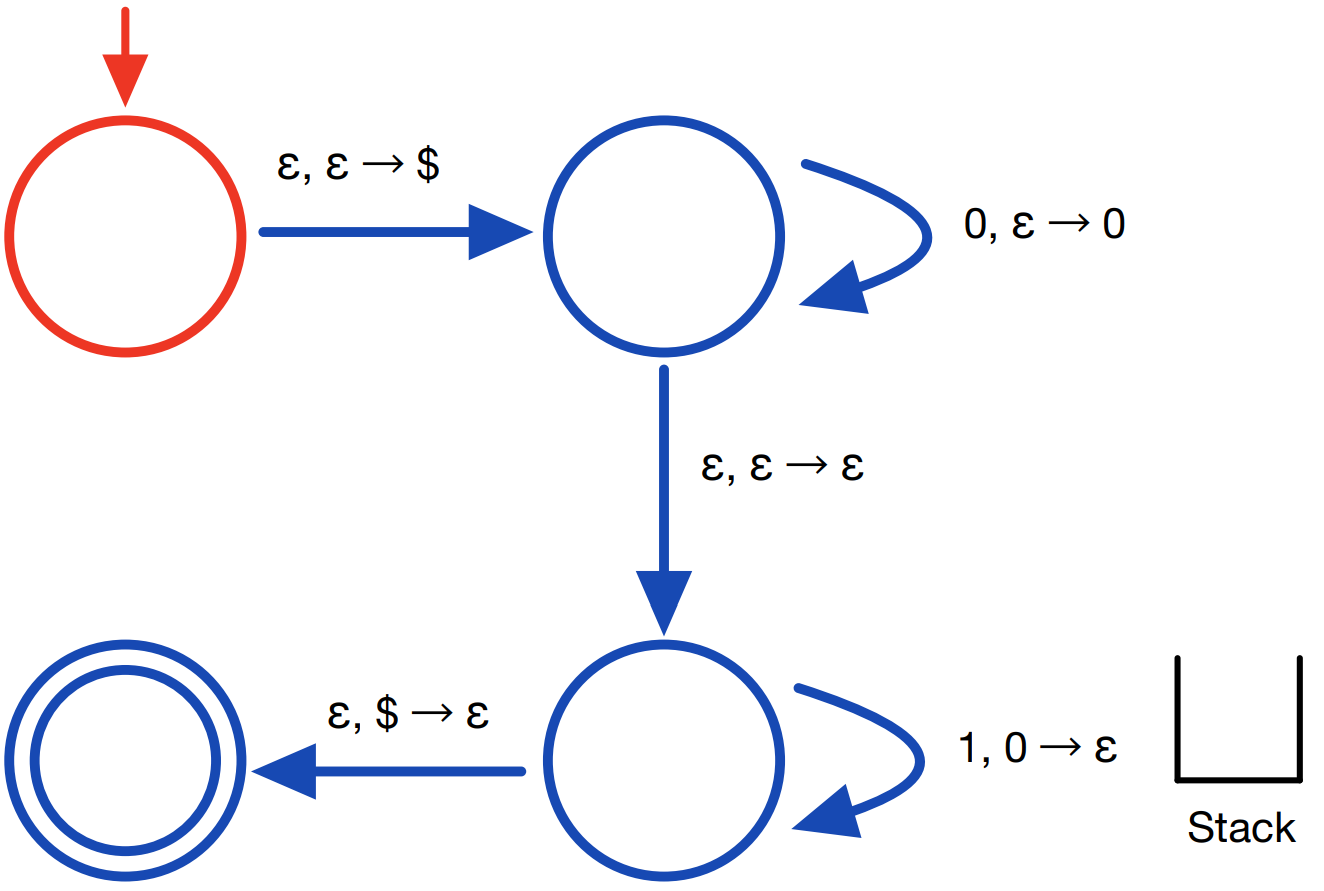
\includegraphics[scale=0.30]{images/pda_comp/PDA_Comp_1.png}
    \end{center}
\end{frame}

\begin{frame}{$\texttt{0011} \stackrel{?}{\in} \Set{0^n 1^n,\ n \geq 0}$}
    \begin{center}
        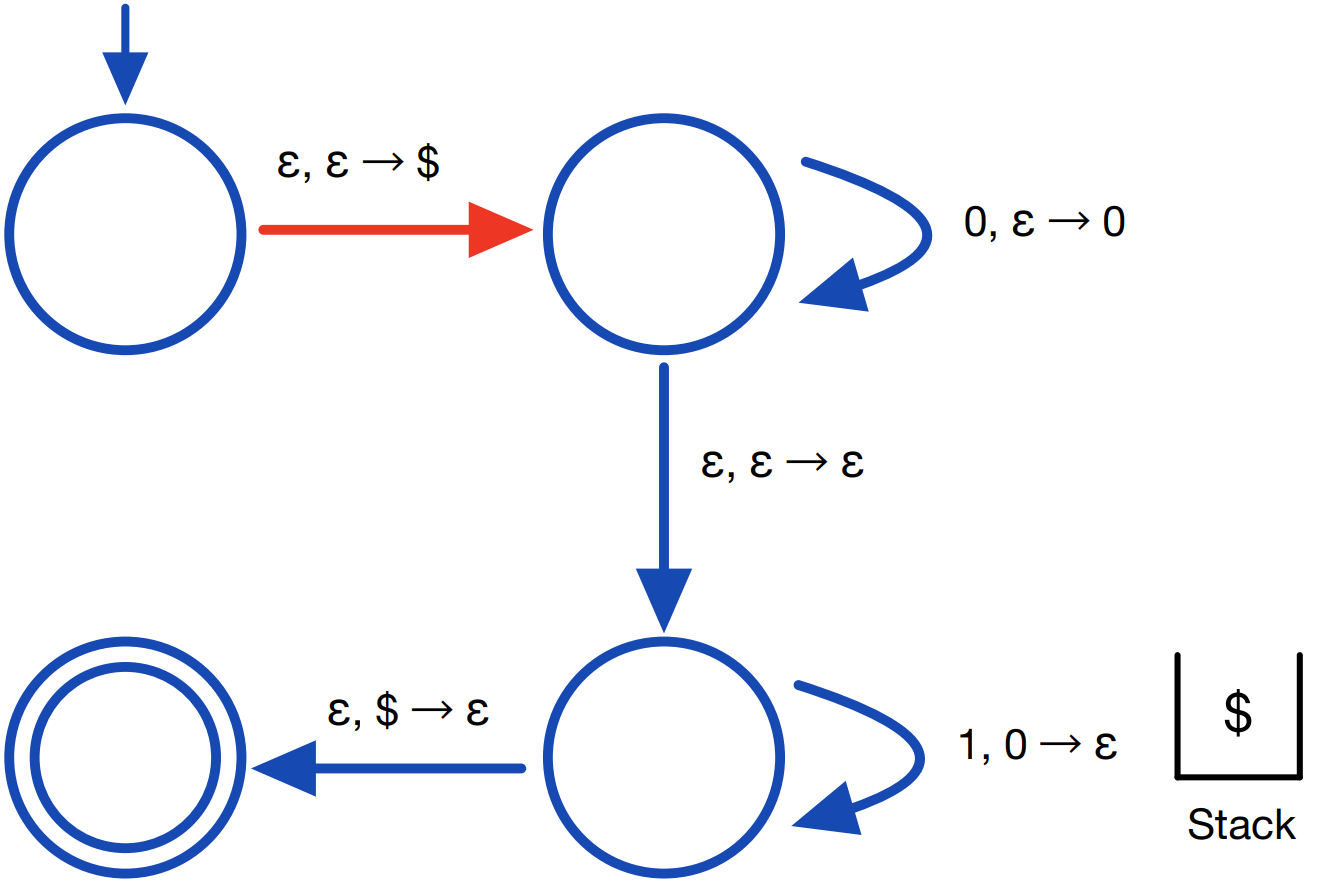
\includegraphics[scale=0.30]{images/pda_comp/PDA_Comp_2.png}
    \end{center}
\end{frame}

\begin{frame}{$\texttt{0011} \stackrel{?}{\in} \Set{0^n 1^n,\ n \geq 0}$}
    \begin{center}
        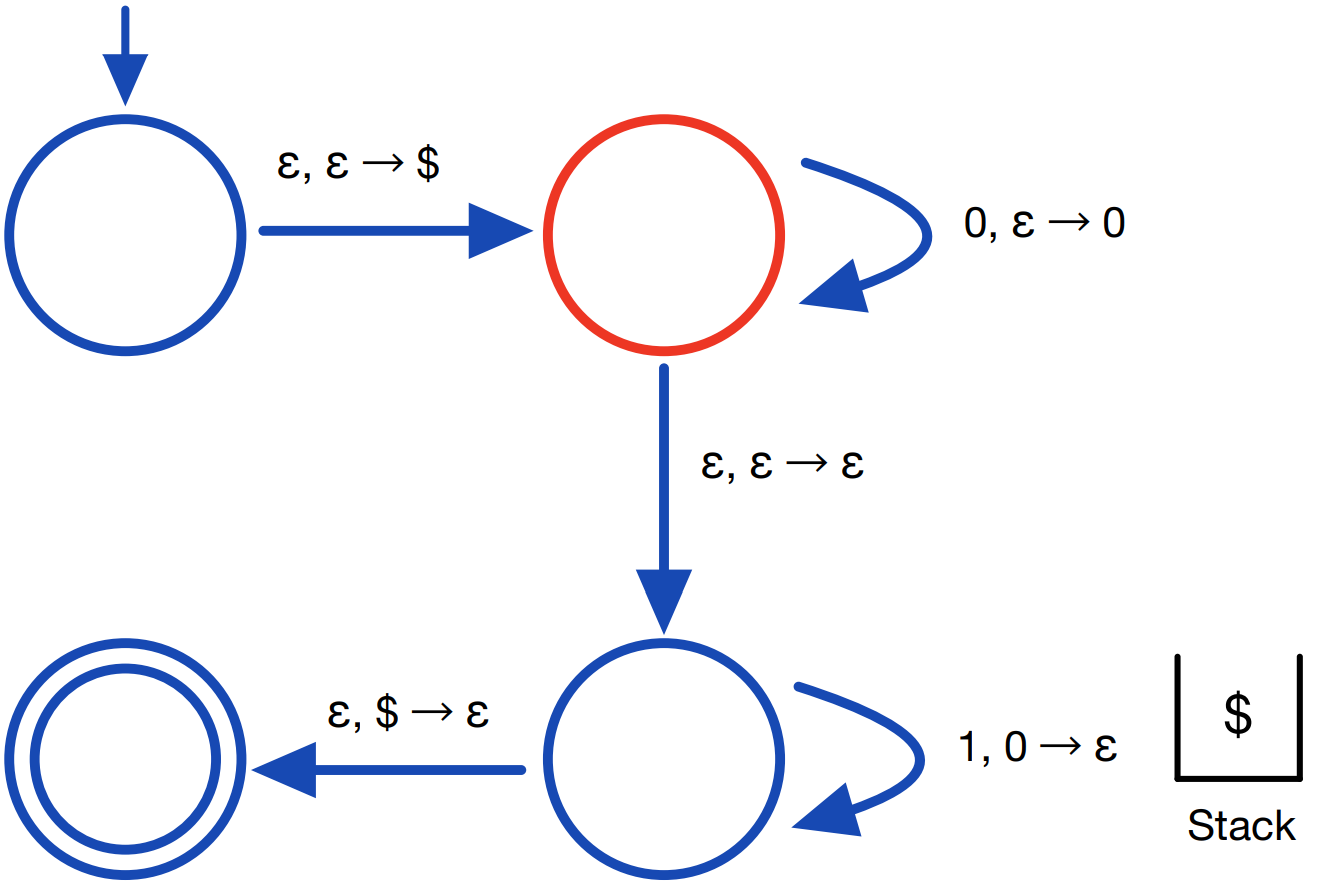
\includegraphics[scale=0.30]{images/pda_comp/PDA_Comp_3.png}
    \end{center}
\end{frame}

\begin{frame}{$\texttt{0011} \stackrel{?}{\in} \Set{0^n 1^n,\ n \geq 0}$}
    \begin{center}
        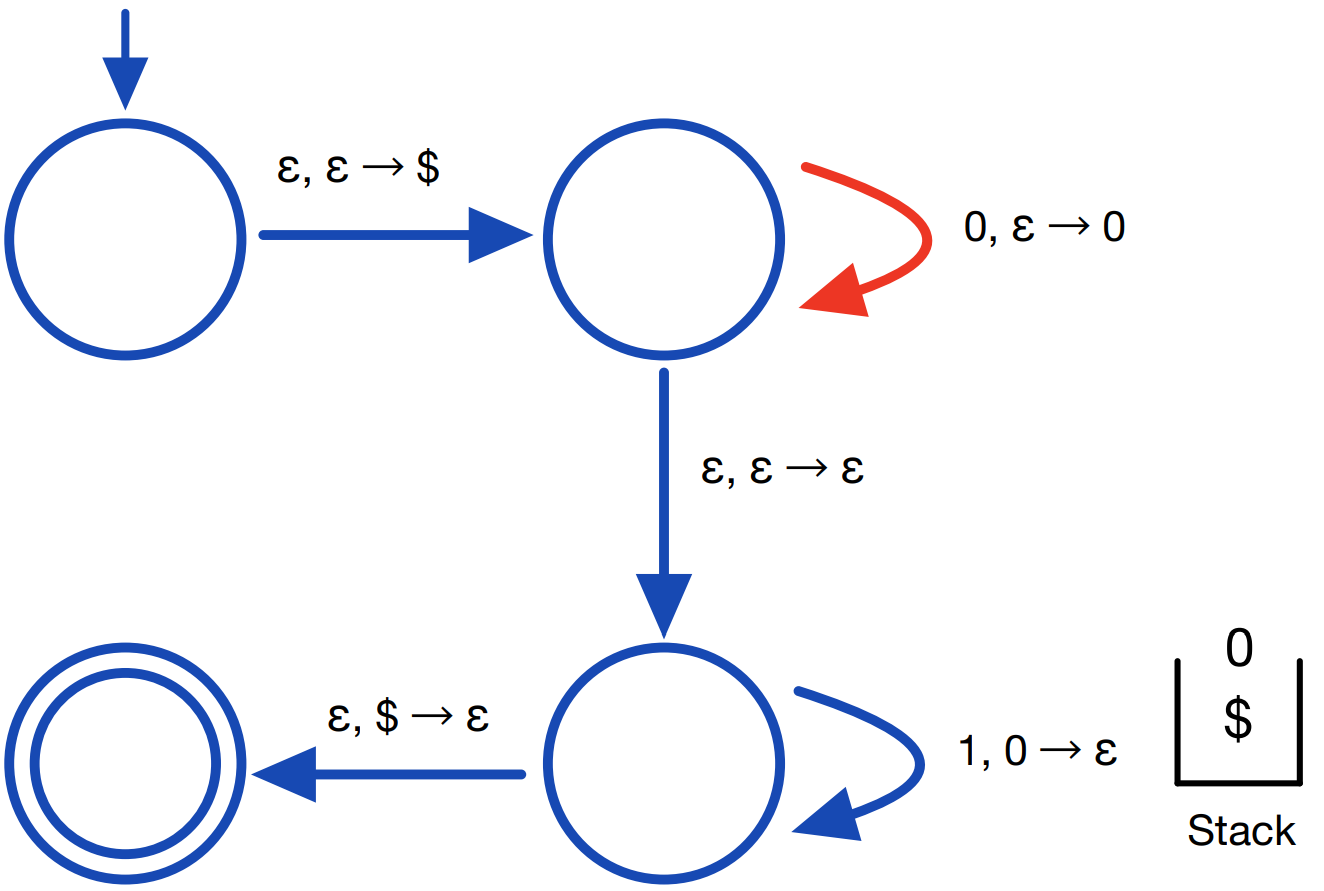
\includegraphics[scale=0.30]{images/pda_comp/PDA_Comp_4.png}
    \end{center}
\end{frame}

\begin{frame}{$\texttt{0011} \stackrel{?}{\in} \Set{0^n 1^n,\ n \geq 0}$}
    \begin{center}
        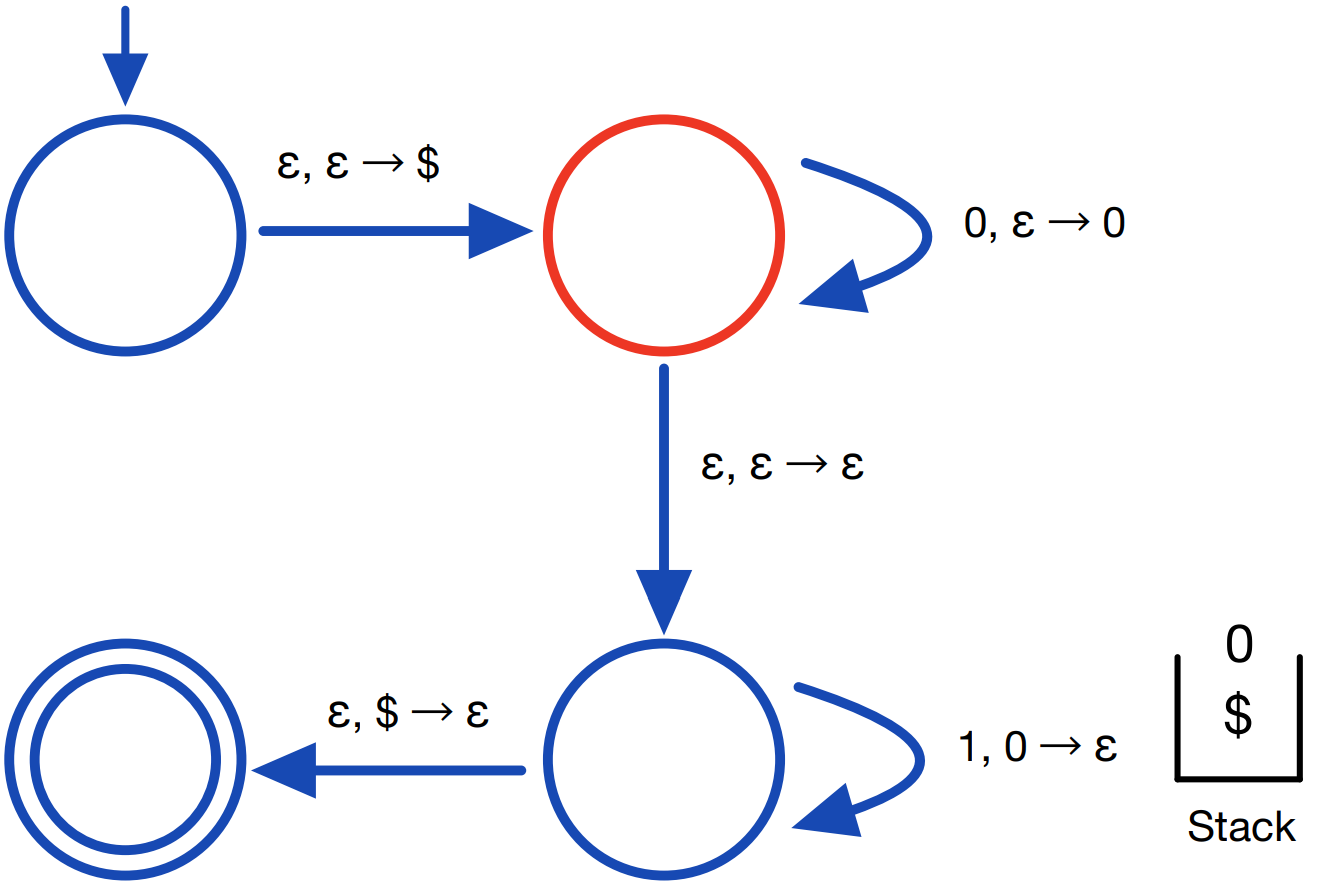
\includegraphics[scale=0.30]{images/pda_comp/PDA_Comp_5.png}
    \end{center}
\end{frame}

\begin{frame}{$\texttt{0011} \stackrel{?}{\in} \Set{0^n 1^n,\ n \geq 0}$}
    \begin{center}
        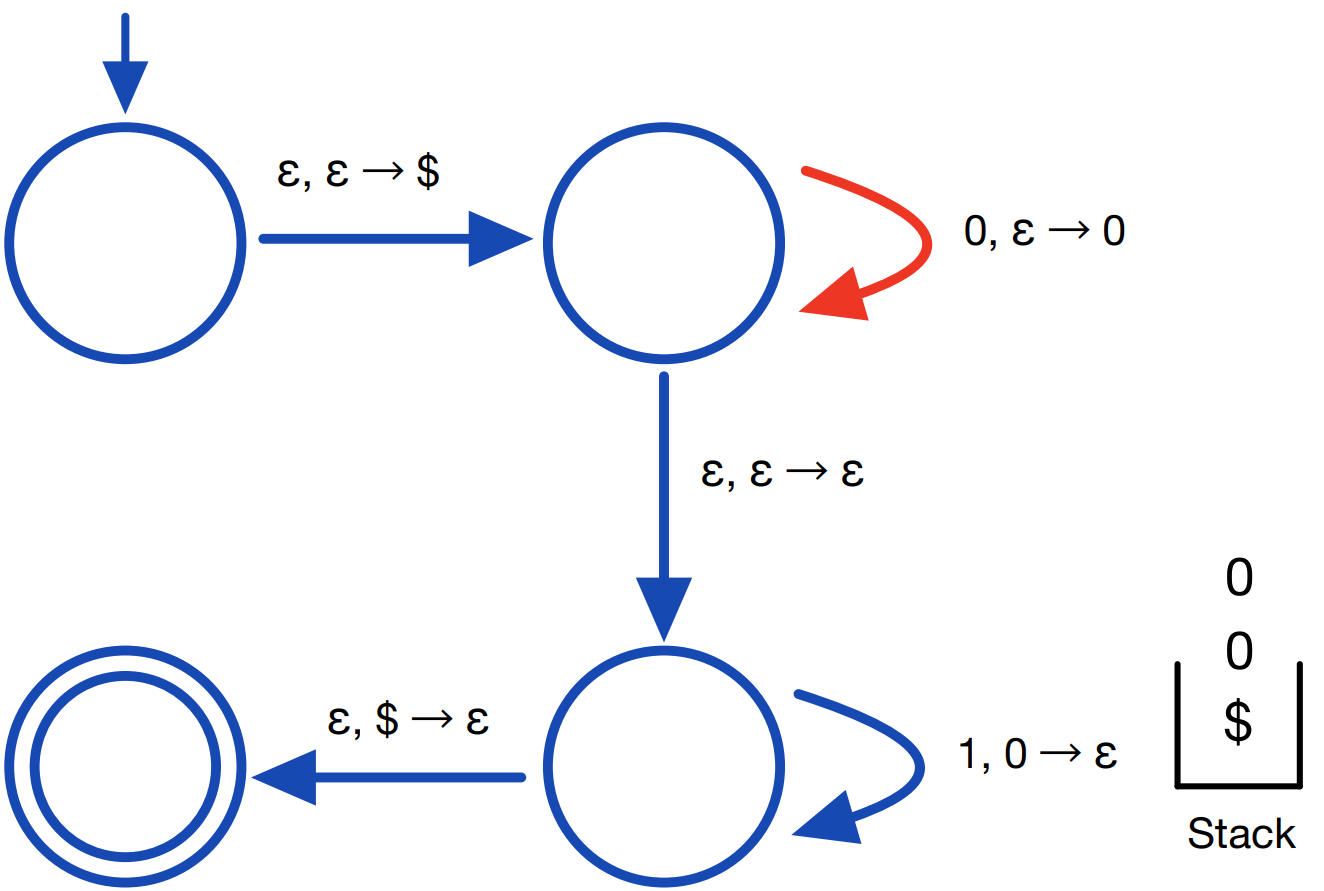
\includegraphics[scale=0.30]{images/pda_comp/PDA_Comp_6.png}
    \end{center}
\end{frame}

\begin{frame}{$\texttt{0011} \stackrel{?}{\in} \Set{0^n 1^n,\ n \geq 0}$}
    \begin{center}
        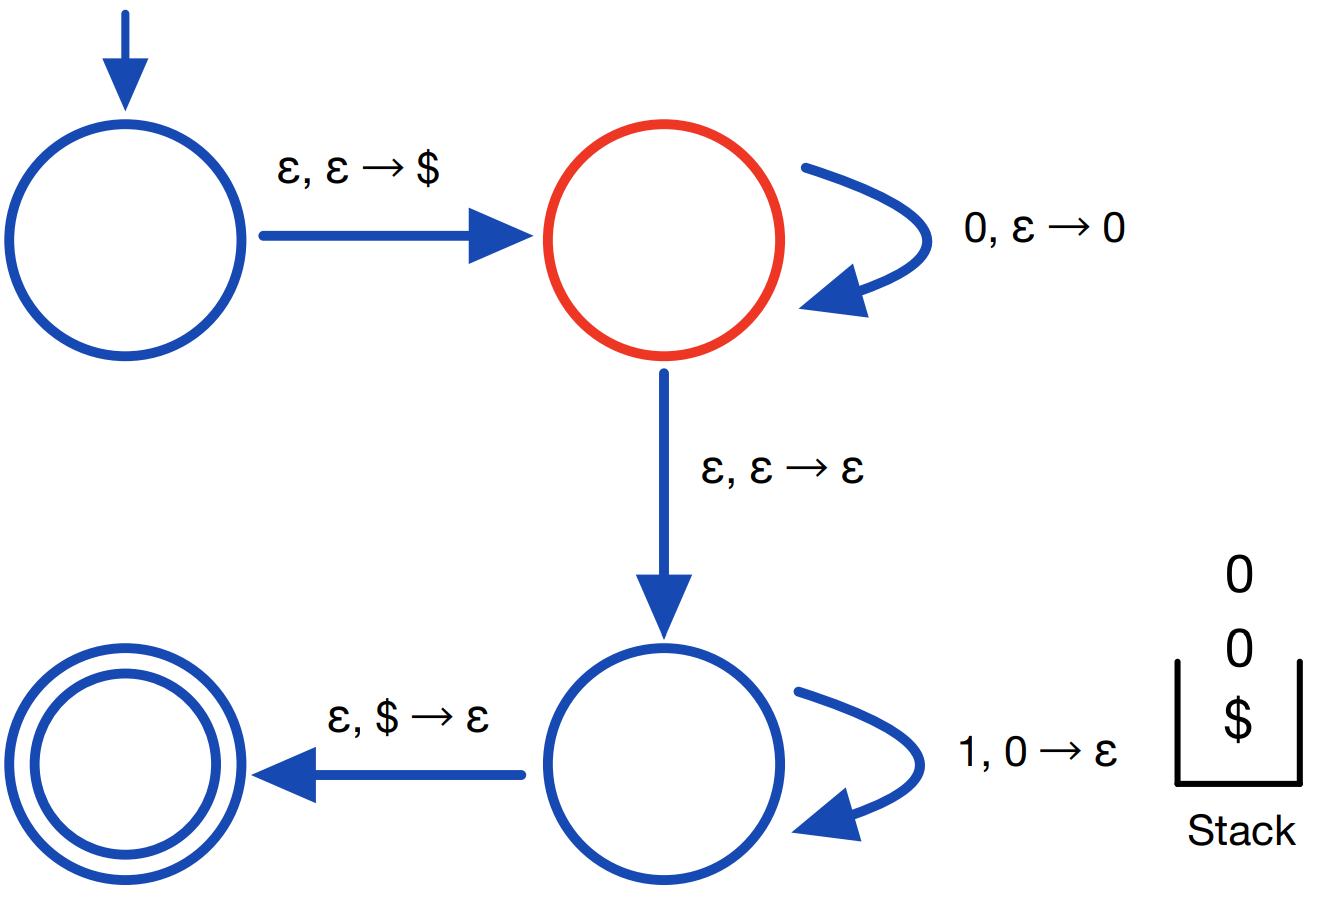
\includegraphics[scale=0.30]{images/pda_comp/PDA_Comp_7.png}
    \end{center}
\end{frame}

\begin{frame}{$\texttt{0011} \stackrel{?}{\in} \Set{0^n 1^n,\ n \geq 0}$}
    \begin{center}
        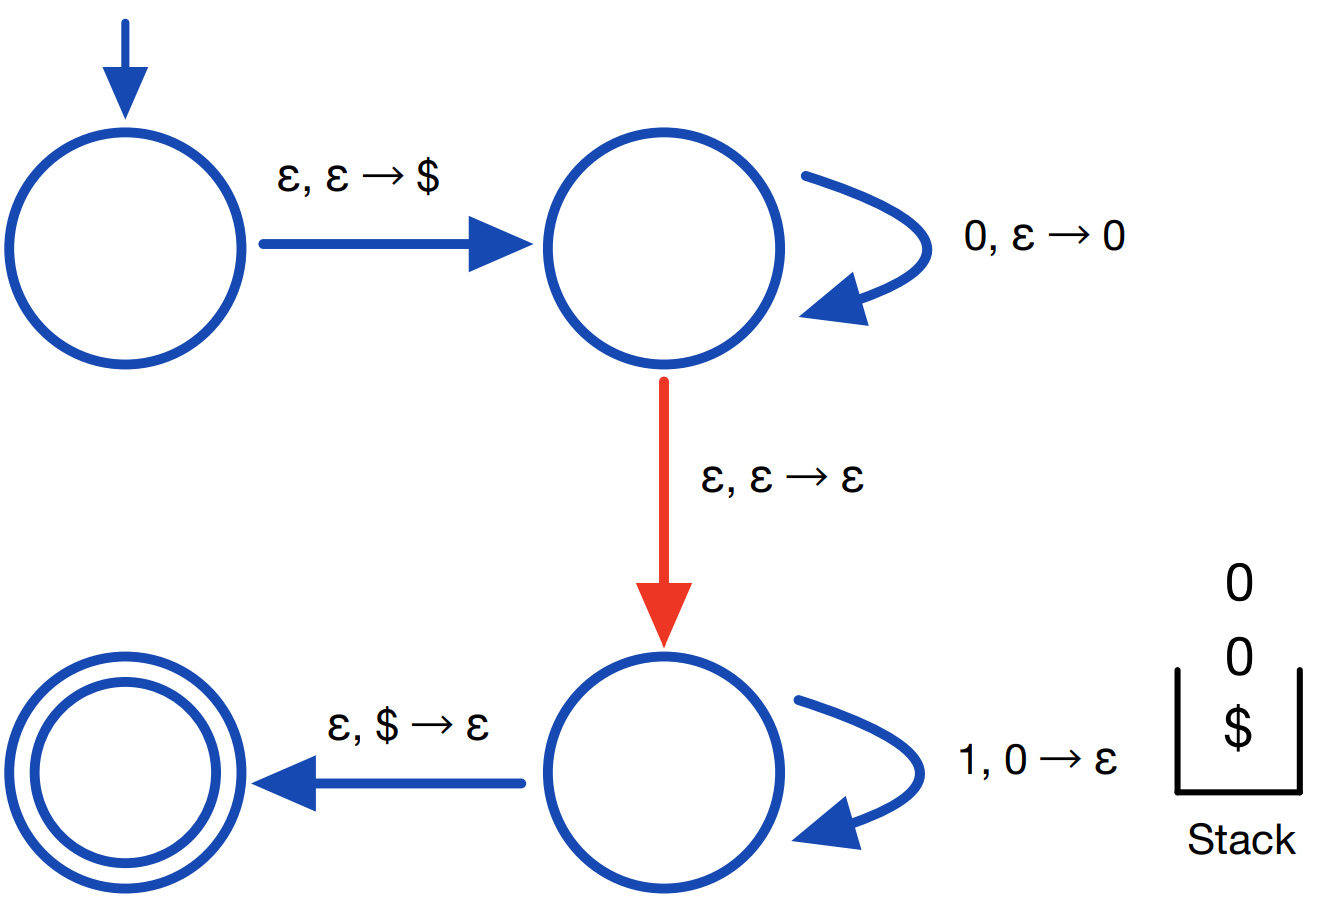
\includegraphics[scale=0.30]{images/pda_comp/PDA_Comp_8.png}
    \end{center}
\end{frame}

\begin{frame}{$\texttt{0011} \stackrel{?}{\in} \Set{0^n 1^n,\ n \geq 0}$}
    \begin{center}
        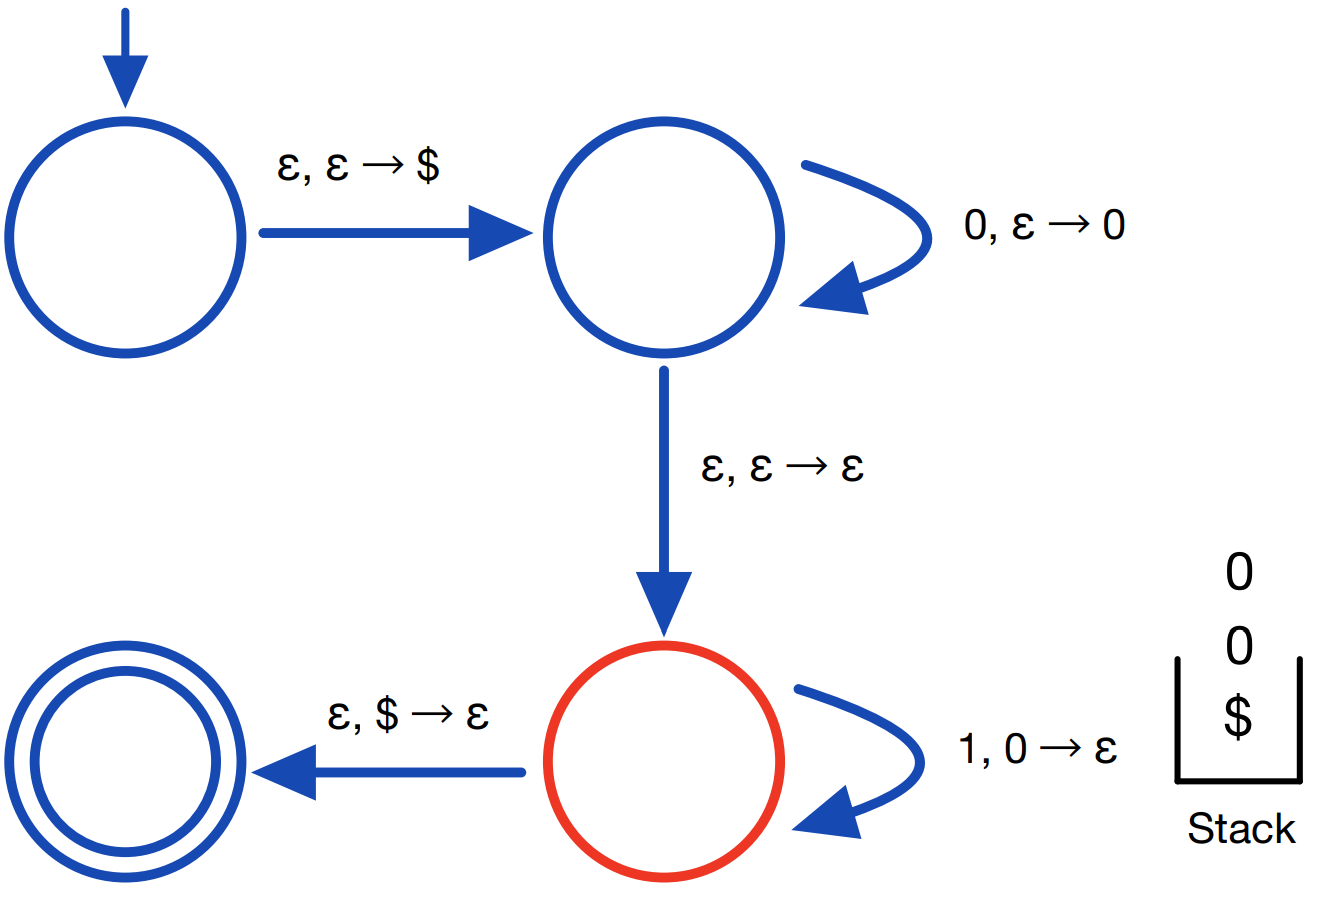
\includegraphics[scale=0.30]{images/pda_comp/PDA_Comp_9.png}
    \end{center}
\end{frame}

\begin{frame}{$\texttt{0011} \stackrel{?}{\in} \Set{0^n 1^n,\ n \geq 0}$}
    \begin{center}
        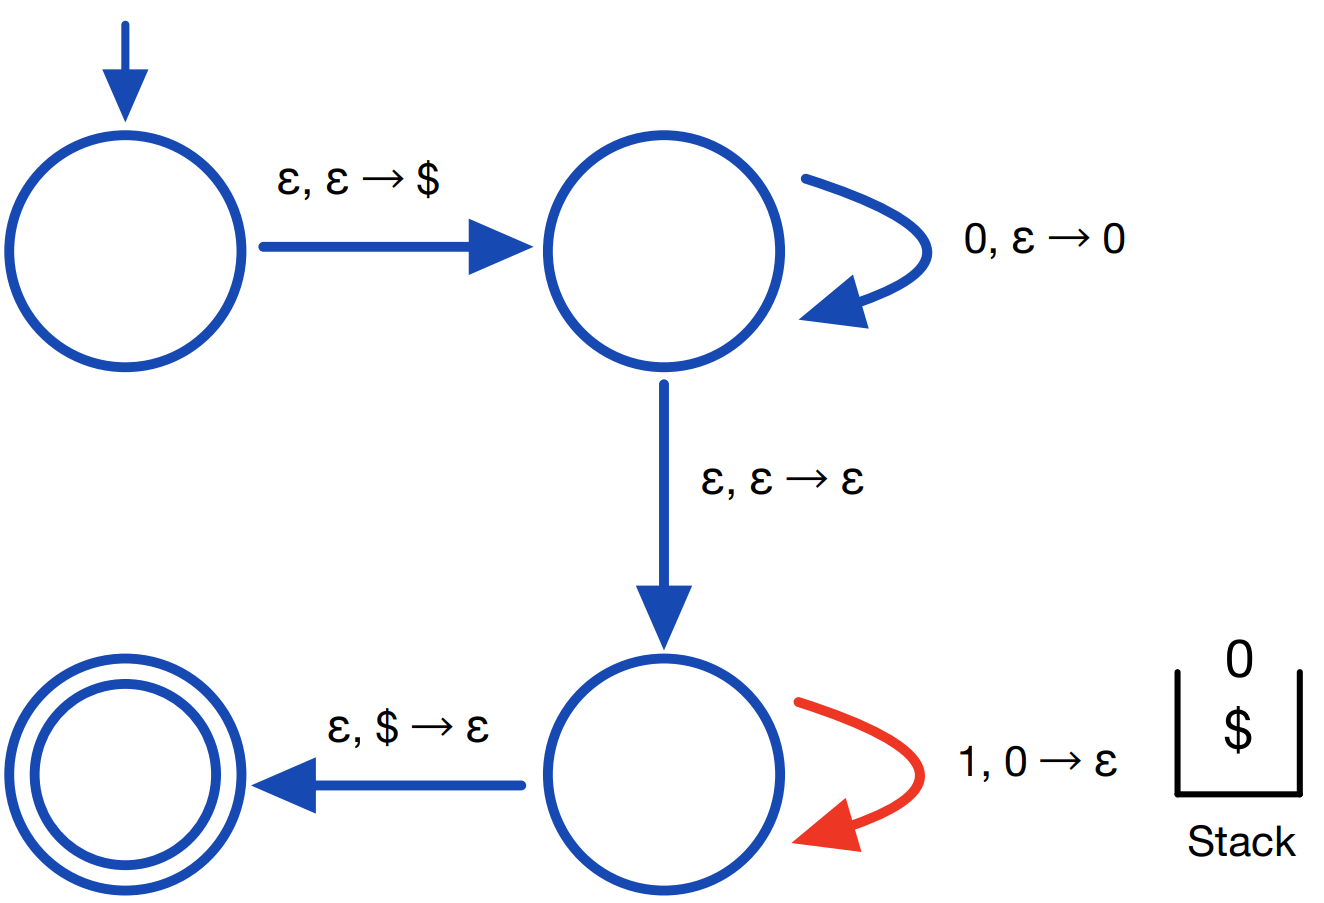
\includegraphics[scale=0.30]{images/pda_comp/PDA_Comp_10.png}
    \end{center}
\end{frame}

\begin{frame}{$\texttt{0011} \stackrel{?}{\in} \Set{0^n 1^n,\ n \geq 0}$}
    \begin{center}
        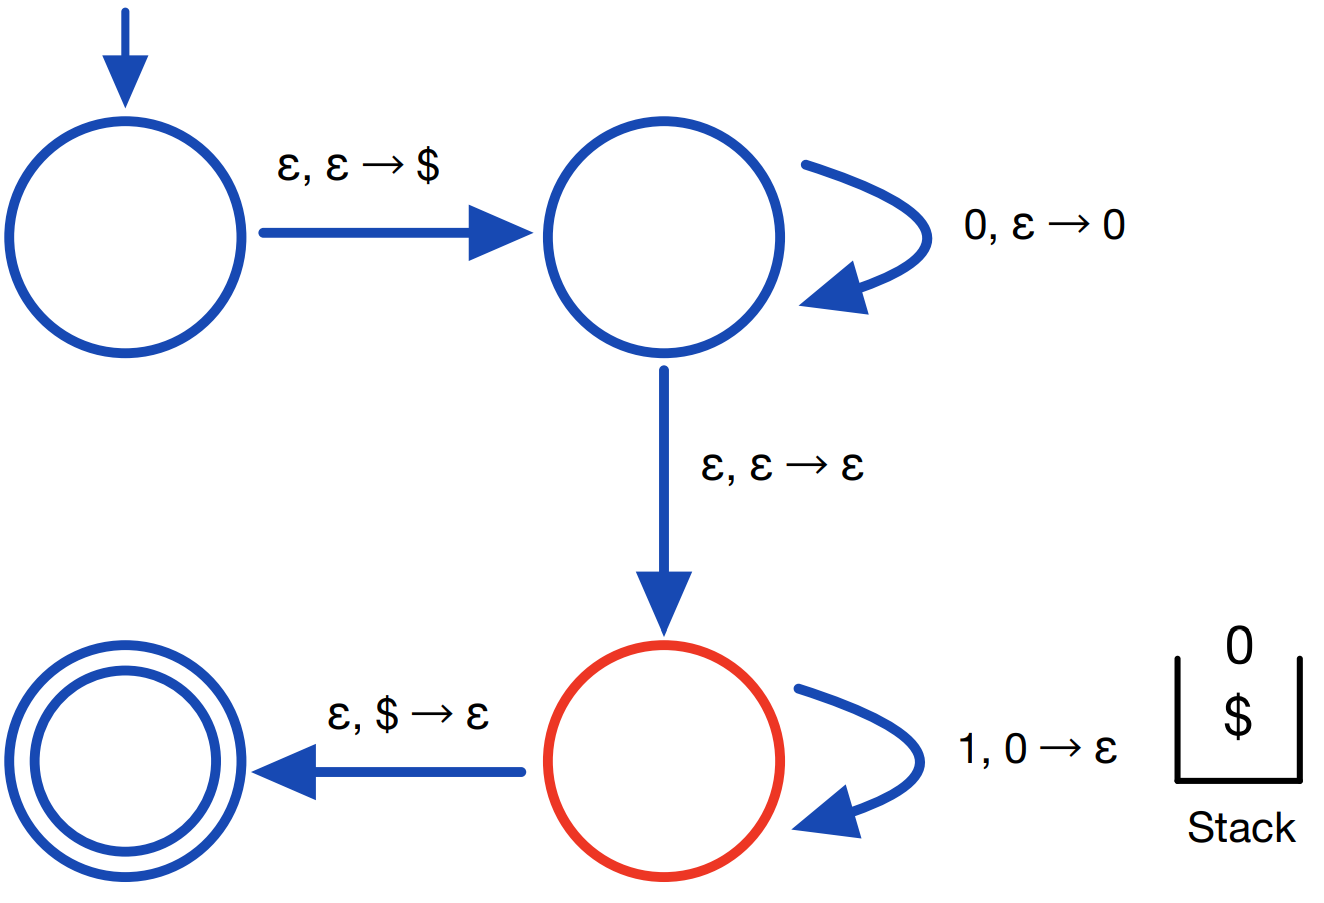
\includegraphics[scale=0.30]{images/pda_comp/PDA_Comp_11.png}
    \end{center}
\end{frame}

\begin{frame}{$\texttt{0011} \stackrel{?}{\in} \Set{0^n 1^n,\ n \geq 0}$}
    \begin{center}
        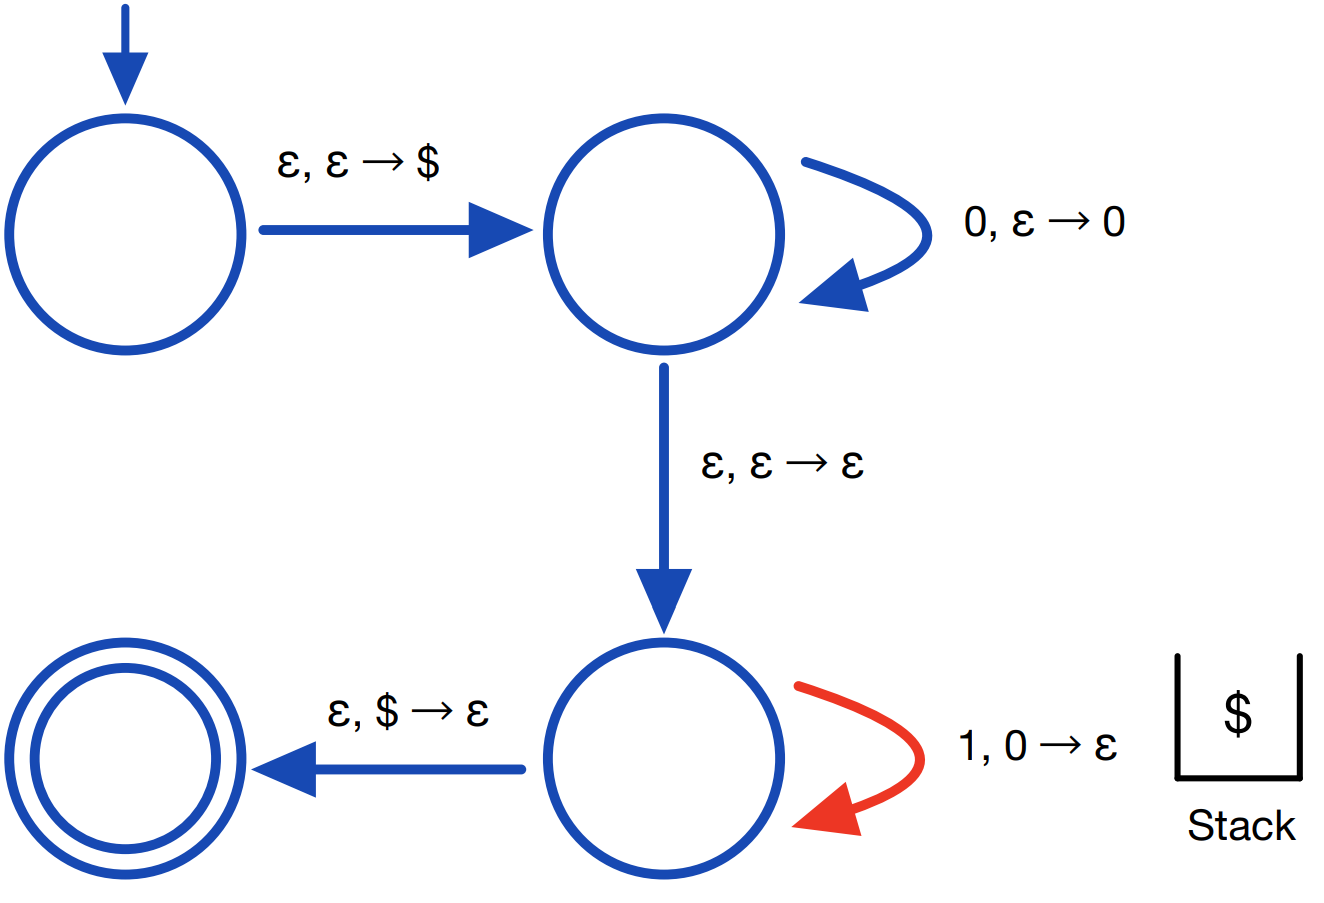
\includegraphics[scale=0.30]{images/pda_comp/PDA_Comp_12.png}
    \end{center}
\end{frame}

\begin{frame}{$\texttt{0011} \stackrel{?}{\in} \Set{0^n 1^n,\ n \geq 0}$}
    \begin{center}
        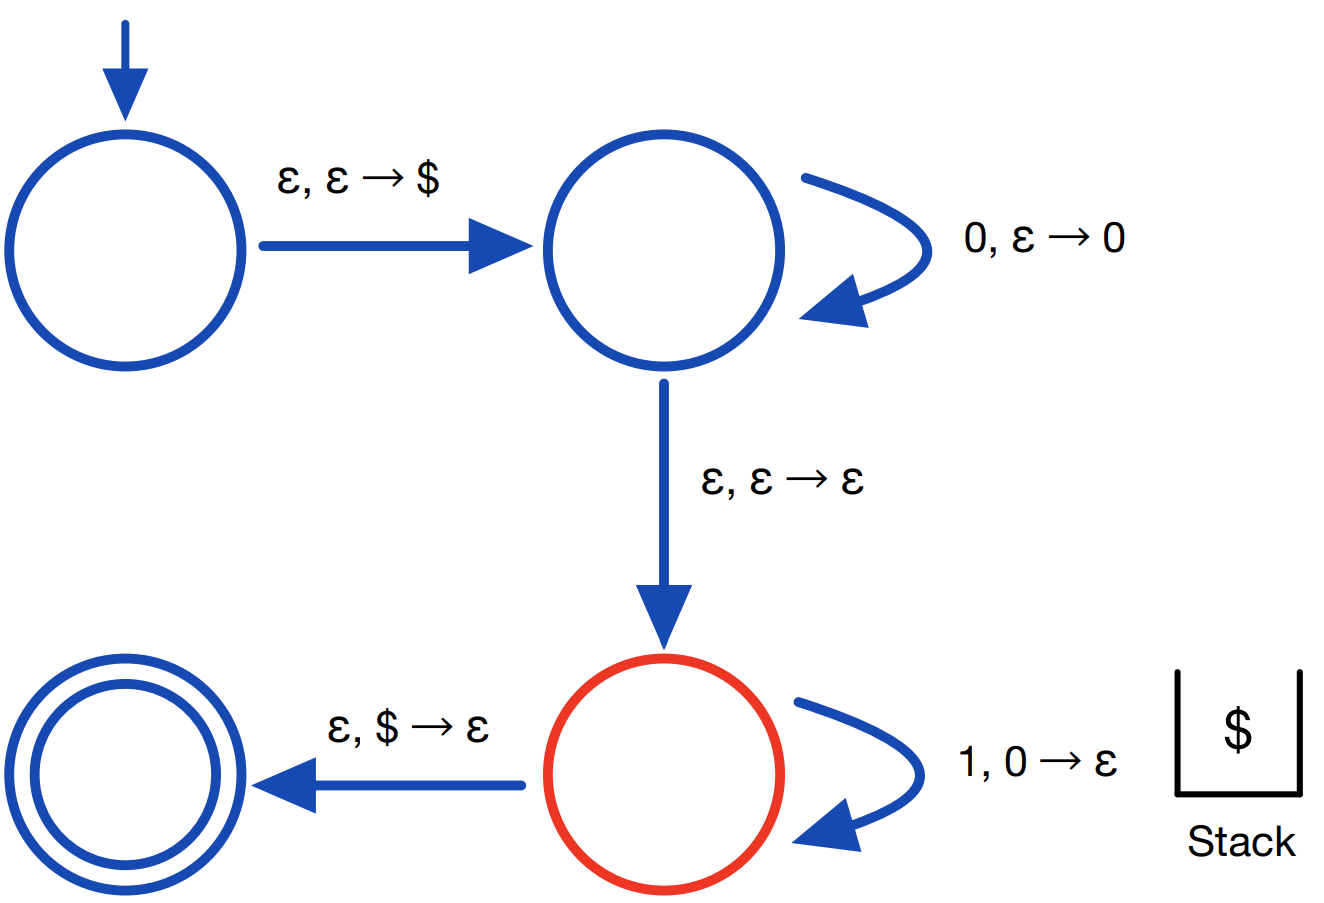
\includegraphics[scale=0.30]{images/pda_comp/PDA_Comp_13.png}
    \end{center}
\end{frame}

\begin{frame}{$\texttt{0011} \stackrel{?}{\in} \Set{0^n 1^n,\ n \geq 0}$}
    \begin{center}
        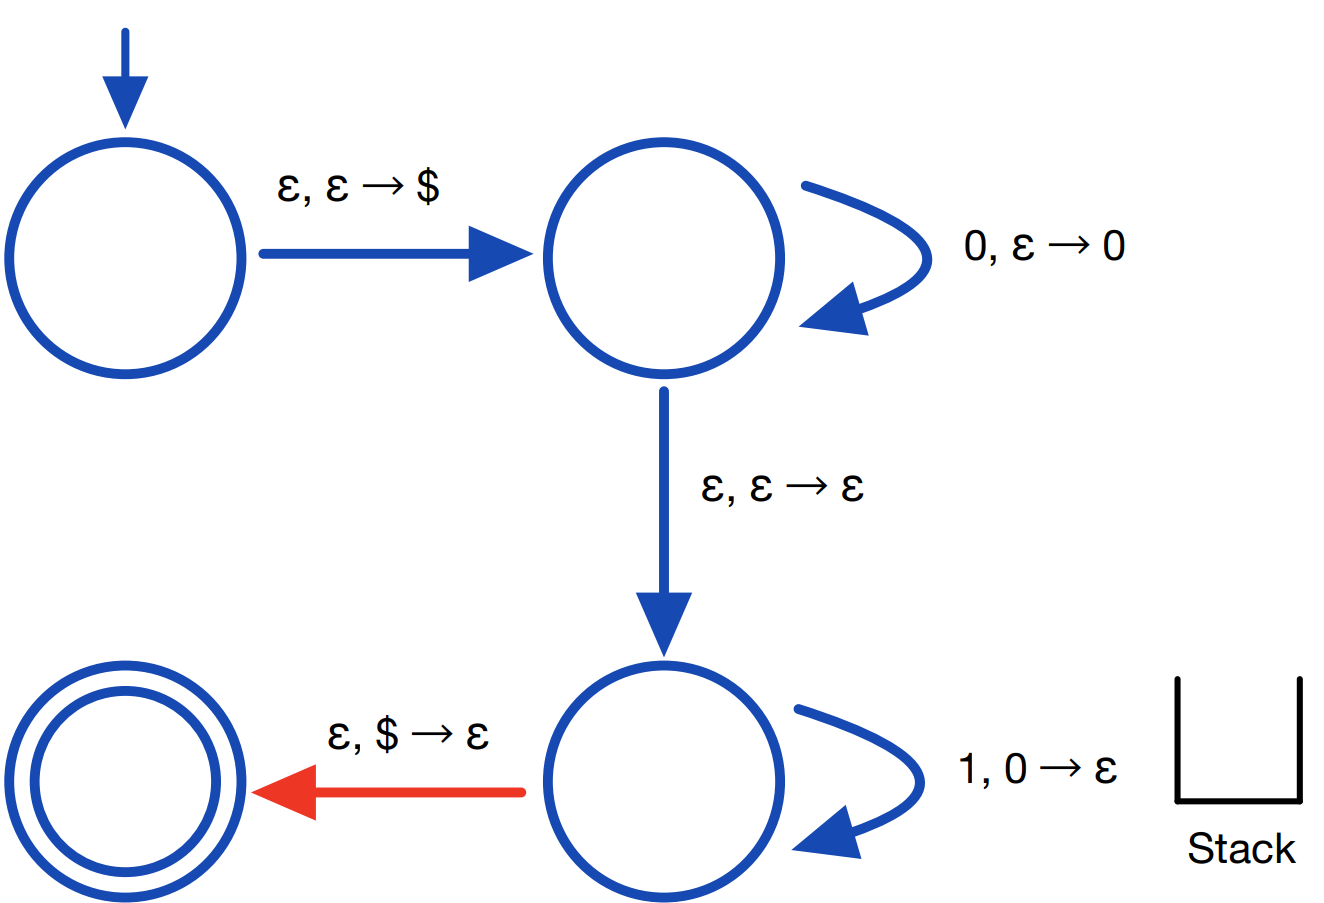
\includegraphics[scale=0.30]{images/pda_comp/PDA_Comp_14.png}
    \end{center}
\end{frame}

\begin{frame}{$\texttt{0011} \stackrel{?}{\in} \Set{0^n 1^n,\ n \geq 0}$}
    \begin{center}
        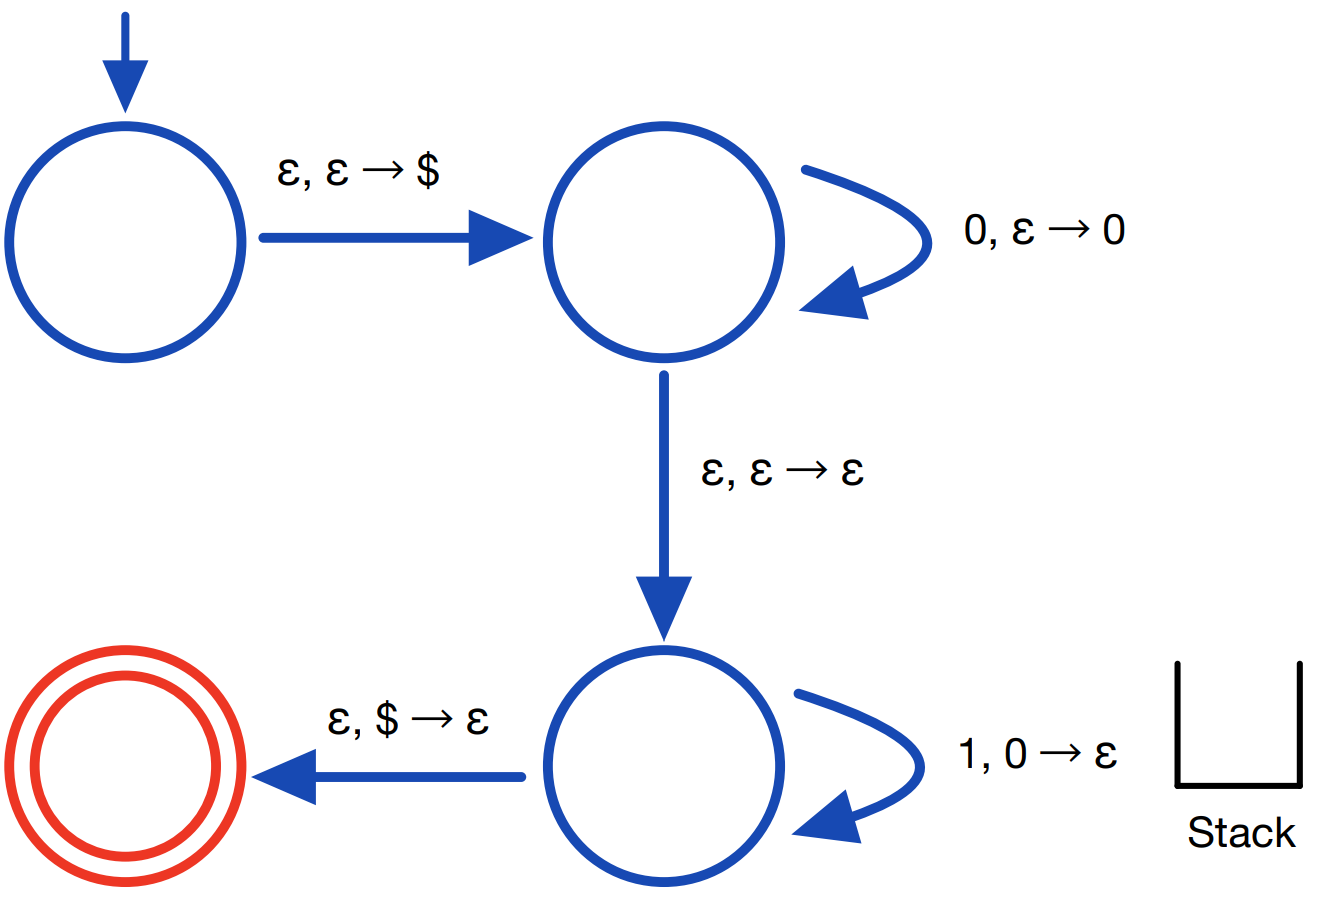
\includegraphics[scale=0.30]{images/pda_comp/PDA_Comp_15.png}
    \end{center}
\end{frame}

\begin{frame}{}
    \begin{center}
        {\color{sigma@mainblue} \LARGE Questions?}
    \end{center}
\end{frame}

\begin{frame}{Questions!}

    \begin{itemize}
        \item Come up with a CFG and a PDA to match the following language 
        $$
            \Set{w | w \text{ has as many \texttt{a}'s as \texttt{b}'s}}
        $$
    \end{itemize}
    
\end{frame}

\begin{frame}{Answers}
    Come up with a CFG and a PDA to match the following language
    $$
        \Set{w | w \text{ has as many \texttt{a}'s as \texttt{b}'s}}
    $$
    {
    \Large
    \begin{align*}
        S ~&\to~ \varepsilon ~|~ S\texttt{a}\texttt{b} ~|~ \texttt{a}S\texttt{b} ~|~ \texttt{a}S\texttt{b}S  \\
    \end{align*}
    }
\end{frame}

\begin{frame}{Answers}
    Come up with a CFG and a PDA to match the following language
    $$
        \Set{w | w \text{ has as many \texttt{a}'s as \texttt{b}'s}}
    $$
    \begin{center}
        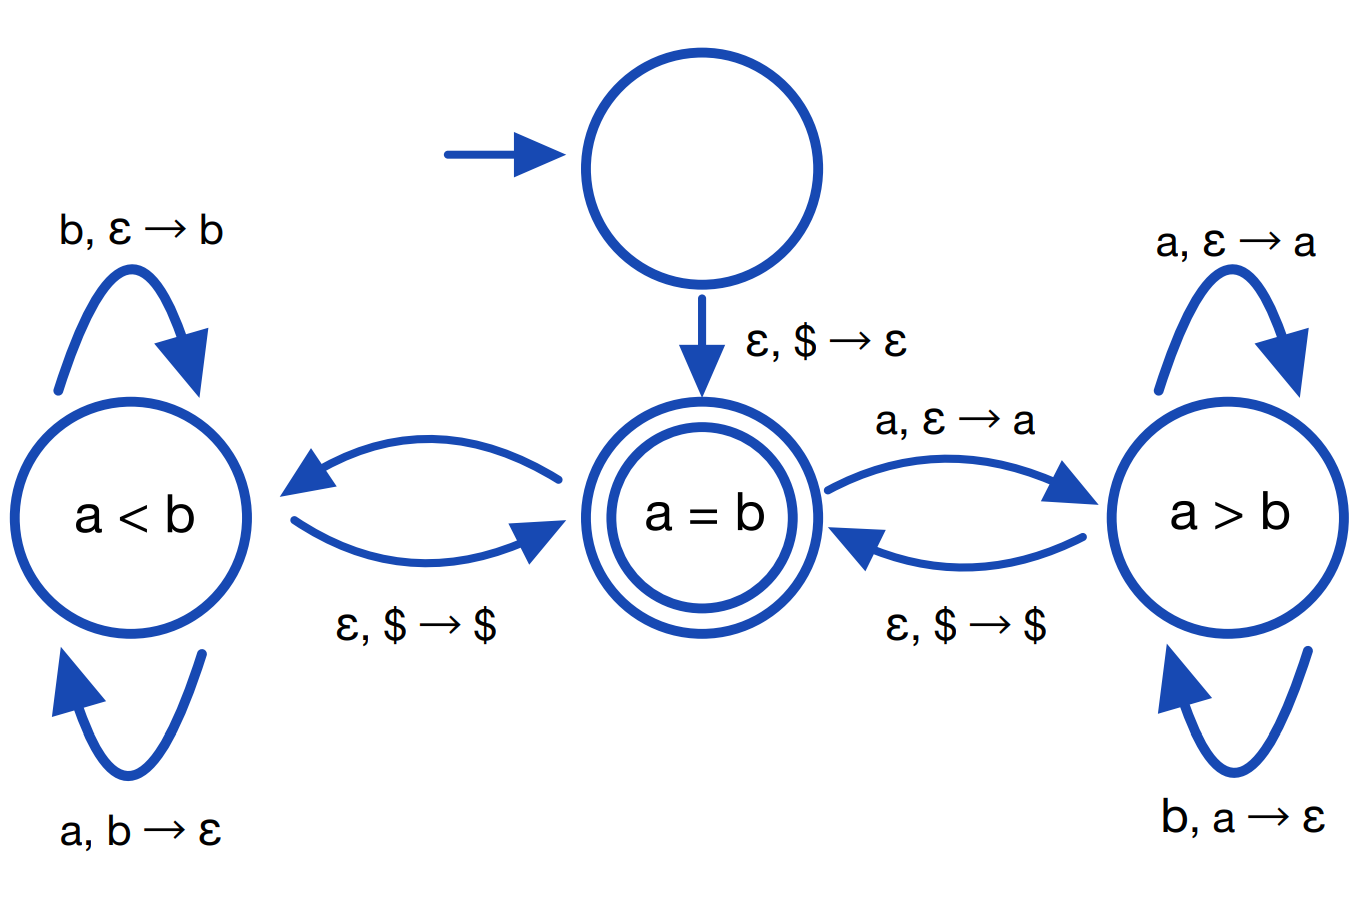
\includegraphics[scale=0.25]{images/wab.png}
    \end{center}
\end{frame}

\end{document}